\chapter{GMC\_NS.jl: Nested sampling by Galilean Monte Carlo for biological models}
\label{chap:GMC}
\path{GMC_NS.jl} implements a basic Galilean Monte Carlo nested sampler \cite{Skilling2012,Skilling2019} in pure Julia. It uses the improved Galilean reflection scheme of Skilling's 2019 GMC publication \cite{Skilling2019}, with increased performance and detailed balance preserved. It uses the natural attrition of model-particles getting stuck in posterior modes to regulate the number of live particles in the model ensemble. This approach partially achieves the same end as algorithms which dynamically adjust the ensemble size based on parameters of the ensemble \cite{Feroz2009,Higson2019}. A minimum ensemble size may be supplied by the user, which is maintained by initializing a new trajectory isotropically from the position of an existing particle; this ensures that the ensemble may be sampled to convergence.

It should be noted that \path{GMC_NS.jl} is a prototype; while it finds posteriors in relatively few iterates, it oversamples less important early regions of the posterior. See \autoref{sec:eggbox} for more information.

\section{Implementation notes}

The basic sampling scheme followed is, first, to initialize an ensemble of models with parameters sampled evenly from across the prior, then to compress the ensemble to the posterior by applying GMC moves to the least-likely model in the ensemble at a given iterate, constrained within its current likelihood contour. GMC tends to move model-particles across the parameter space evenly and efficiently, particularly in the initial portion of compression across the uninformative bulk of the prior mass. That said, GMC particles may get "stuck" in widely separated minima, so there are instances when the least-likely particle has no valid GMC moves. In this case, the trajectory is not continued. Instead, the trajectory is removed from the ensemble and sampling continues, unless the number of particles in the ensemble would decline below the specified minimum. In this case, a new trajectory is begun by resampling from the remaining prior mass within the ensemble. This is accomplished by random ``diffusive" proposals, in contrast to the ordinary, directed Galilean movements. A random particle remaining within the ensemble is selected, and isotropic velocity vectors are sampled from this particle to find a starting location for the new trajectory (this vector is conferred to the new particle).

\path{GMC_NS.jl} follows the common convention of transforming parameter space to a unit-standardized hypersphere ("unit ball"). The density of the prior is uniform, that is $\pi(x) = 1$, over the -1:+1 range of the hypersphere dimension. Utility functions \path{to_unit_ball} and \path{to_prior} transform prior coordinates to the unit ball, and unit ball positions to the prior coordinate, respectively. In future versions, this scheme is likely to be modified to a 0:1 unit hypercube, which does not require operations beyond obtaining the cumulative probability of a parameter value on the prior distribution. The user may also specify a sampling "box" to bound particles from illegal or nonsensical areas of the parameter space (eg. negative values for continuous distributions on positive-valued physical variables). The box reflects particles specularly in the same manner as the likelihood boundary, with the exception that because the orientation of the $n$th-dimensional box "side" is known, the reflection is performed by stopping the particle at the box side and giving it reversing its velocity vector in dimension $n$. 

\path{GMC_NS.jl} attempts to maintain efficient GMC sampling by per-particle PID tuning of the GMC timestep. GMC treats models as particles defined by their parameter vectors, which give their positions in parameter space, and a velocity vector, initalised isotropically and only changed when the particle "reflects" off the ensemble's likelihood contour. In GMC, when a model-particle is moved through the parameter space (in this case, because it is the least likely particle in the ensemble), a new position is proposed by extending some distance along its velocity vector. This distance is determined by scaling the velocity vector by a "timestep" value, which defines the per-iterate rate at which the particle traverses the parameter space. As the model ensemble is compressed to the posterior, this timestep must decline in order for proposals to be acceptable, as the amount of available parameter space declines rapidly. Additionally, GMC particles may enter convoluted regions of parameter space that form small likelihood-isthmuses to other, more likely regions. In order to deal with this, each trajectory is assigned its own PID tuner, which maintains an independent timestep value for the trajectory. The PID algorithm is tuned to target an unobstructed move rate. In short, PID tuning will reduce the timestep if the particle is frequently reflecting off the likelihood boundary (in which case it is crossing the remaining prior mass without sampling much from within it, or it is in a highly convoluted area of the local likelihood surface), and extend the timestep if it the particle frequently moves without encountering the boundary, so that particles that are closely sampling an open region without encountering the boundary begin to "speed up".

PID constants and default GMC settings have been crudely tuned to produce the best possible result with the stated sampling scheme on the eggbox problem, as described in \autoref{sec:eggbox}.

\section{Ensemble, Model, and Model Record interfaces}
In operation, \path{GMC_NS.jl} maintains a \path{GMC_NS_Ensemble} mutable struct in memory. The directory to which the sampler ought to save the ensemble is specified by its \path{path} field. \path{GMC_NS.jl} does not maintain calculated models in memory, instead serializing them to this directory. In order to track the positions and likelihoods of model-particles within the ensemble and as samples from the posterior, a \path{GMC_NS_Ensemble} maintains two vectors of \path{GMC_NS_Model_Records} as fields; \path{models} for live particles, and \path{posterior_samples} for the previous positions along trajectories. Observations against which models are being scored, prior distributions on model parameters, model constants (if any), and the sampling box are specified by the \path{GMC_NS_Ensemble}'s \path{obs}, \path{priors}, \path{constants}, and \path{box} fields, respectively. The \path{GMC_NS_Ensemble} also specifies settings for the GMC sampler and the PID tuner. Sensible defaults for these values may be passed (usually, splatted) en masse to an ensemble constructor with the \path{GMC_DEFAULTS} constant exported by \path{GMC_NS.jl}.

Therefore, to use \path{GMC_NS.jl} with their model, the user must write a model-appropriate version of these three structs (the ensemble, model, and model record) with the fields specified by the docstrings in the \path{/src/ensemble/GMC_NS_Ensemble.jl} file, as well as \path{/src/GMC_NS_Model.jl}. The user is responsible for an appropriate constructor and likelihood function for the model, any required parameter bounding functions, and so on. The user may optionally write a overloaded \path{Base.show(io::IO, m::GMC_NS_Model)} function for displaying the model, or a \path{Base.show(io::IO, m::GMC_NS_Model, e::GMC_NS_Ensemble)} function for displaying the model with observations or other ensemble data. This function can be used with the package's \path{ProgressMeter} displays for on-line monitoring of the current most likely model.

\section{Usage notes}
\subsection{Setting up for a run}
Given an appropriately coded model, as outlined above, the user must define a number of important values for the sampler before a \path{GMC_NS_Ensemble} may be constructed. These values are stored in fields of the ensemble. Firstly, the user must prepare the observation data in whatever format is suitable for the model's likelihood function. Next, one must define a vector of \path{Distribution}s on parameters of the model as the \path{prior} field of the ensemble. These must be univariate, as the CDF of the distribution is used to determine position on that dimension. Some functions to produce univariate marginal distributions from multivariate Normal Gamma and Normal Inverse Gamma priors are available in \path{NGRefTools.jl}. Next, any constants used in the likelihood function must be available in the \path{constants} field of the ensemble. A \path{box} matrix with $n$-dimensional rows containing minimum and maximum values in the first and second columns defines the maximum extent of parameter space to be explored. The sampler expects the box in the transformed hypercoordinates mentioned above; a one-dimensional box across the entire prior would be \path{[-1 1]}. It is convenient to compose the matrix in the original parameter space and perform the transformation with a broadcast call to \path{to_unit_ball()}, either in the ensemble constructor or in the calculation script.

\subsection{GMC and PID tuner settings}
The GMC sampler is governed by settings specified in \path{GMC_NS_Ensemble} fields. These include the PID tuner settings, and are summarized below:

\path{GMC_Nmin} (Integer; Default $50$): The minimum number of active model-particles in the ensemble. After the initial sample from the prior, new particles will only be generated when required to maintain this value. Otherwise, when a valid proposal cannot be found for the current least-likely trajectory (i.e. the PID tuner drives the timestep below \path{GMC_}$\tau$\path{_death}), the nested sampling step consists of removing that particle to the posterior samples and moving on to the next live particle, without replacement. 

\path{GMC_}$\tau$\path{_death} (Float; Default $1e-5$): Value of trajectory's $\tau$ timestep, below which the particle is considered to be dead. A dead particle's trajectory is not continued. This value is denominated in hypersphere coordinates. If this value is very small ($\leq 1e-6$), trajectories may carry on for thousands of iterates in relatively unimportant regions.

\path{GMC_init_}$\tau$ (Float; Default $1.$): Initial value of the timestep for all trajectories. This applies to the particles assembled on ensemble construction; particles generated from diffusional resampling inherit the $\tau$ of their parent, but with the isotropic vector which generated the proposal for their new location.

\path{GMC_tune_}$\mu$ (Integer; Default $4$): Length of tuner memory; the proposal acceptance rate $\alpha$ is calculated over the previous $\mu$ constructor reports for this trajectory. Tends to produce oversampling if it is much more than 10.

\path{GMC_tune_}$\alpha$ (Float; Default $.25$): Target acceptance rate for proposals. Sampler efficiency benefits from this being fairly low (.2-.4).

\path{GMC_tune_PID} (NTuple{3,Float}; Default ($.3$,$0.$,$0.$)): kP, kI, and kD constants for the tuner. kP can be somewhat larger. kI and kD are probably detrimental when using short tuner memory, but could be useful if an efficient longer memory regime is available.

\path{GMC_timestep_}$\eta$ (Float; Default $.25$): If this value is >0., a normally distributed error with a standard devation of $\tau \cdot $\path{GMC_timestep_}$\eta$ is applied to $\tau$ before calculating the GMC proposals, as suggested by \cite{Skilling2012}.

\path{GMC_reflect_}$\eta$ (Float; Default $.005$: If this value is >0., it is used to perturb reflection vectors, as suggested by \cite{Skilling2012}. It is applied to sampling box reflections as well as likelihood contour reflections. It should be a small value. If it is too large, sampling box reflections can ``bend'' the wrong way and produce an inappropriate series of samples at the box boundary.

\path{GMC_exhaust_}$\sigma$ (Float; Default $10.$): Scale factor multiplied into ensemble size to determine the maximum number of unsuccessful searches to perform before terminating sampling. This virtually never happens.

\path{GMC_chain_}$\kappa$ (Integer, Default typemax(Int64)). Number of iterates at which to terminate a sampling chain/trajectory. By default, this does not occur. Can prevent oversampling in some cases.


\subsection{Parallelization}
\path{GMC_NS.jl} does not have an explicit parallelization scheme; the sampler proceeds linearly to the next least-likely particle and performs the appropriate Galilean trajectory sampling procedure. Parallelization may nonetheless be achieved at two levels; the likelihood function may be parallel according to the needs of the user, and individual nested sampling runs may be arbitrarily combined. That is, if one desires to parallelize a \path{GMC_NS.jl} job, it is best to think in terms of the total number of trajectories to be sampled, dividing this by the number of machines available to perform the sampling work, to obtain the number of particles to be sampled on each machine. The sampling runs can then be combined post hoc to achieve the desired final accuracy. In this scheme, the likelihood function is best parallelized by threading on a single machine.

\subsection{Displays}
Parameters of the ensemble and most-likely model can be monitored on-line, while \path{GMC_NS.jl} is working. This is done by specifying a vector of function vectors (ie a \path{Vector{Vector{Function}}}). One such vector may be supplied to specify the displays to be shown above the \path{ProgressMeter}, one for those below, supplied as the \path{upper_displays} or \path{lower_displays} keyword arguments to \path{converge ensemble!()}. \path{GMC_NS.jl} will rotate the upper and lower displays to the next vector of display functions every \path{disp_rot_its} sampling iterates, supplied as another \path{converge_ensemble!()} keyword argument. Default display functions are available in \path{/src/utilities/progress_displays.jl} and are exported for easy composition of the function vectors.

\subsection{Eggbox diagnostic}
The ``eggbox test'' is a toy model designed by Feroz et al. \cite{Feroz2009}, and used by others for use in characterising nested sampling algorithms \cite{Buchner2016}. It uses the likelihood function $logL = (2 + cos(5π \cdot x1) \cdot cos(5π \cdot x2))^5$. This function has 18 optima and a canonical logZ evidence score of 235.88. The most efficient solution to this problem is afforded by MultiNest; it accurately sums the model evidence in approximately 10000 iterates with 400 particles. \path{GMC_NS.jl} correctly finds the 18 optima of the eggbox, and converges in fewer iterates, as displayed in \autoref{eggboxfig}. However, it substantially underestimates the model's evidence; typical \path{GMC_NS.jl} logZ evidence estimates for the eggbox are consistently ~229. This tendency to systematically underestimate the evidence should be kept in mind when examining the evidence estimates in this thesis.

% \begin{figure}[!h]
%     \makebox[\textwidth][c]{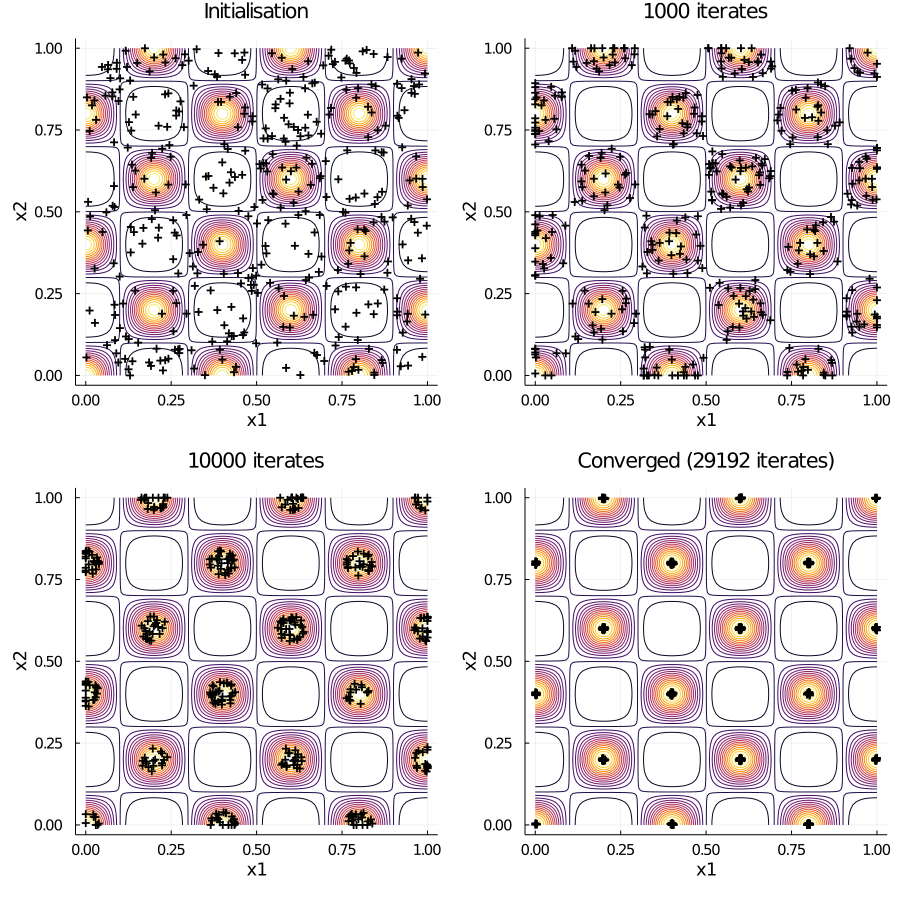
\includegraphics{GMC/eggbox.png}}    
%     \caption{{\bf \path{GMC_NS.jl} nested sampling the eggbox toy model}
%     \label{eggboxfig}
% \end{figure}

The eggbox may be estimated with the following code:

\begin{minted}[breaklines,
    mathescape,
    linenos,
    numbersep=5pt,
    frame=lines,
    framesep=2mm]{julia}
    using GMC_NS, Distributions

    #compose priors
    prior=Uniform(0,1); priors=[prior,prior]

    #sampling box
    box=[-1. 1.
         -1. 1.]

    #monitor convergence
    lds=Vector{Vector{Function}}([[ensemble_display]])

    #terminate slowly moving particles
    gmc=copy(GMC_DEFAULTS)
    gmc[2]=1e-3

    #assemble 400 particle ensemble
    e=Eggbox_Ensemble("eggbox_test", 400, priors, box, gmc...)

    #converge the ensemble
    converge_ensemble!(e,backup=(true,100), lower_displays=lds, converge_factor=1e-6)
\end{minted}

which produces the following output:

\subsection{Example use}
\path{GMC_NS.jl} is supplied with two simple, but useful, statistical models by default. These are the \path{Normal_Model} and \path{LogNormal_Model} subtypes of \path{GMC_NS_Model}. Users may familiarize themselves with \path{GMC_NS.jl}'s operation by the use of these models. A simple demonstration is supplied in the \path{/test} directory of the package. The program is detailed with additional comments below. The demonstration involves converging an ensemble of 10 \path{Normal_Model} chains initialized from an inaccurate \path{NormalGamma} prior on data generated from a known \path{Normal} distribution.

\begin{minted}[breaklines,
    mathescape,
    linenos,
    numbersep=5pt,
    frame=lines,
    framesep=2mm]{julia}
#Import dependencies
using GMC_NS, Distributions, ConjugatePriors

#Generate some data from a Normal model with \mu 100. and \sigma 5. 
sample_dist=Normal(100.,5.)
samples=rand(sample_dist, 10000)

#An inaccurate ConjugatePrior
prior=NormalGamma(300.,2e-3,1.,10.) 

#Box for the two parameters of the Normal model.
#First column: parameter minimums.
#Second column: parameter maximums
#First row: \mu
#Second row: precision, ie 1/sqrt(\sigma)
#eps() is machine epsilon, ~1e-16; a small number
box=[0. 1000.
     1/1000. 1/eps()]

#Start with the default sampler settings
#Index 1: Lower the minimum number of ensemble particles to 5
#Index 2: The minimum allowable particle timestep is set to a very small number; the likelihood of the model parameterisation can be determined precisely and is well behaved over the parameter space.
gmc=GMC_DEFAULTS
gmc[1]=5
gmc[2]=1.e-15

#Assemble the ensemble. Begin with 10 particles
e=Normal_Ensemble("NE_test", 10, samples, prior, box, gmc...)

#Define the upper displays to be rendered above the status line. Here we rotate a single display between three readouts.
uds=Vector{Vector{Function}}([[convergence_display],[evidence_display],[info_display]])

#Define the lower displays to be rendered below. We want to look at the most likely model in the ensemble plotted against the observations the whole time.
lds=Vector{Vector{Function}}([[model_obs_display]])

#Converge the ensemble, serializing to pwd/NE\_test every 100 iterates and rotating the chosen displays every 1000 iterates.
converge_ensemble!(e,backup=(true,100),upper_displays=uds, lower_displays=lds, disp_rot_its=1000)
\end{minted}

Typical output after executing this program is presented in \autoref{GMCnormoutput}. The maximum a priori parameters may be read off the $\theta$ line of the \path{model_obs_display} below the status line. The algorithm estimates that the model from which the sample was drawn has a $\mu$ of $\sim$ 100.29 and a precision of $\sim$ .045, corresponding to a $\sigma$ of $\sim$ 4.7; the global optimum has been found despite the poor starting prior.

\begin{figure}[!h]
    \makebox[\textwidth][c]{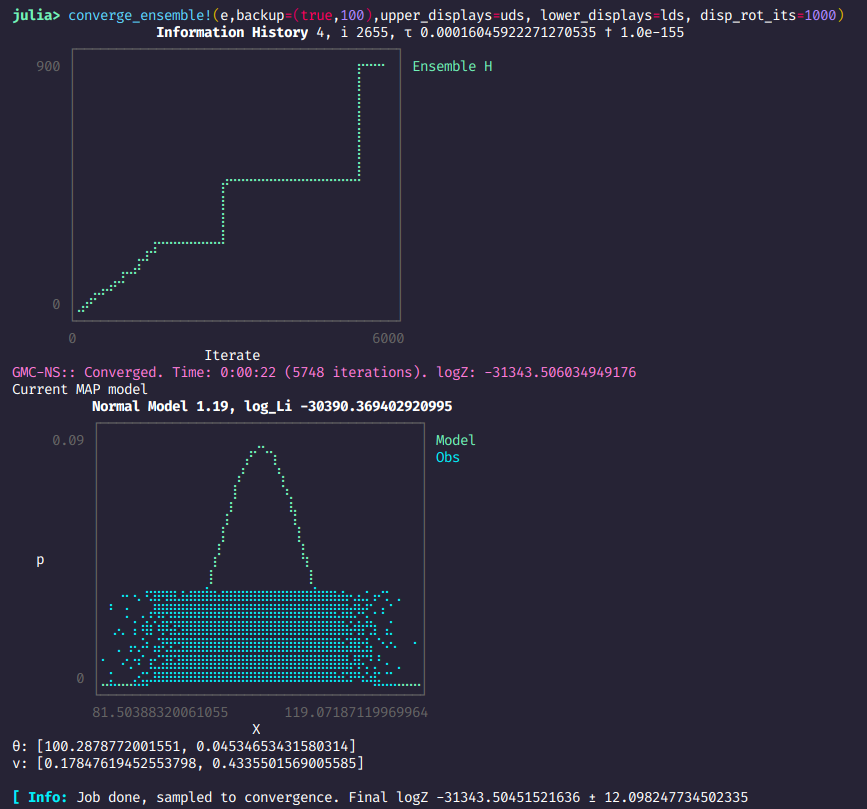
\includegraphics{BMI/output.png}}    
    \caption{{\bf Example \protect\path{BMI.jl} Output}}
    \label{GMCnormoutput}
\end{figure}

\section{Future Directions}

\path{GMC_NS.jl} could be improved in at least three ways. Firstly, it ought to be trajectory- or sampling chain-centric rather than ensemble-centric, so that ensembles can be dynamically assembled in the manner suggested by Speagle \cite{Speagle2020}, which might fix the evidence accuracy problem this sampler exhibits. Secondly, an ellipsoidal search routine has been coded for \path{GMC_NS.jl}, but remains to be implemented; this could be used to initialize new chains in a dynamic sampling routine. Lastly, the GMC PID tuning system likely needs improvement. pI an pD constants are largely superfluous, and there may be a more fundamentally justified way to confer the information supplied by boundary contact to the particle by way of timestep tuning.